

\begin{frame}{Myonen-Tomographie}

		\begin{block}{Die Idee}
			\begin{itemize}
			 	\item benutze kosmische Myonen, um 2D/3D Aufnahmen von Volumina zu erstellen
		  		\item Myonen durchdringen Materie viel weiter als z.B. Photonen
		  		\item Bestimmung von Spur und Energieverlusten, um massive Körper zu untersuchen
		  		$\rightarrow$ Suche nach Dichteunterschieden
			\end{itemize}
		\end{block}
		
		\begin{block}{Beispiele}
			\begin{itemize}
			 	\item Louis Alvarez' Untersuchung der Chephren-Pyramide, Ägypten, um versteckte Räume zu
			 	finden: Platzierung einer Funkenkammer in unterem Geschoss (60er)
			 	\item Untersuchung von Magmakammer von Vulkanen, um Eruptionen vorhersagen zu können
			 	(Szintillatoren oder Halbleiterdetektoren)
			 	\item zukünftig: Untersuchung der Kernschmelzen der Fukushima Reaktoren
			\end{itemize}
		\end{block}
\end{frame}

\begin{frame}{Myonen-Tomographie}
\begin{columns}[T]
		\column{.6\textwidth}
			\begin{figure}[htbp]
			  \centering
			  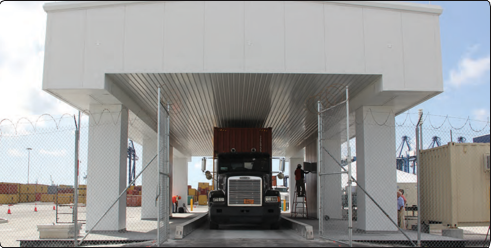
\includegraphics[width=0.8\columnwidth]{bilder/beispiele/muoncargo}
			\end{figure}
			\vspace{-0.3cm}
				\begin{figure}[htbp]
			  \centering
			  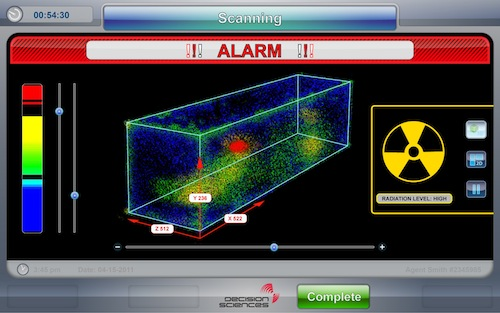
\includegraphics[width=.8\columnwidth]{bilder/beispiele/muondetected}
			  \caption*{[gds]}
			\end{figure}
		\hspace{1cm}
		\column{.5\textwidth}
		
		\begin{itemize}
		  \item Untersuchung von Transportern/Schiffsfracht hauptsächlich auf Kernwaffenmaterial
		  \item Streuung kosmischer Myonen an schweren Kernen $\rightarrow$ Rekonstruktion der
		  Dichteverteiung in Volumen durch Messung der Spuren der Myonen
		  \item Spurdetektoren: z.B. Szintillationsdetektoren und Driftkammern (Drift tubes)
		\end{itemize}
    \end{columns}
\end{frame}